\section{Architecture matérielle et chaînes RF d’un SAR embarqué}\label{SEC:Architecture matérielle et chaînes RF d’un radar SAR embarqué}

\subsection{Architecture fonctionnelle globale}

\subsubsection{Architecture radar}

Il existe plusieurs architectures matérielles possibles pour un radar en fonction de plusieurs paramètres, du contexte et du coût. Comme cité précédemment, le radar génère des impulsions d'énergie RF de courte durée et de forte puissance qui sont rayonnées dans l'espace par l'antenne. Suite au rayonnement de l'onde par l'environnement, le récepteur radar reçoit un signal atténué et bruité avant d'être traité. 
L'émetteur radar doit présenter les caractéristiques techniques et opérationnelles suivantes :
\begin{enumerate}
    \item L'émetteur doit être capable de générer la puissance RF moyenne requise et la puissance de crête requise;
    \item L'émetteur doit avoir une bande passante RF appropriée;
    \item L'émetteur doit présenter une stabilité RF élevée afin de répondre aux exigences en matière de traitement du signal;
    \item L'émetteur doit être efficace, fiable et facile à entretenir, et la durée de vie et le coût du dispositif de sortie doivent être acceptables.
\end{enumerate}
Le récepteur radar doit présenter les caractéristiques techniques et opérationnelles suivantes :
\begin{enumerate}
  \item Le récepteur doit posséder une sensibilité suffisante pour détecter des signaux de faible puissance provenant de cibles éloignées;
  \item Le récepteur doit avoir une bande passante adaptée à la largeur spectrale du signal émis afin d'assurer une détection correcte;
  \item Le récepteur doit présenter un faible facteur de bruit pour maximiser le rapport signal sur bruit;
  \item Le récepteur doit être doté d'une dynamique élevée afin de gérer des signaux de puissance variable;
  \item Le récepteur doit offrir une stabilité de fréquence et de phase élevée pour garantir la cohérence du traitement du signal;
  \item Le récepteur doit permettre un traitement efficace du signal reçu (filtrage, amplification, conversion, numérisation, etc.);
  \item Le récepteur doit être efficace, fiable et facile à entretenir, et la durée de vie et le coût du dispositif de sortie doivent être acceptables.
\end{enumerate}

L'architecture varie dépendamment de tous ces facteurs, le choix de la forme d'onde impacte notemment les chaines RF. Ci-dessous, deux exemples de schéma blocks de radar FMCW et pulse.

\begin{figure}[h]
    \centering
    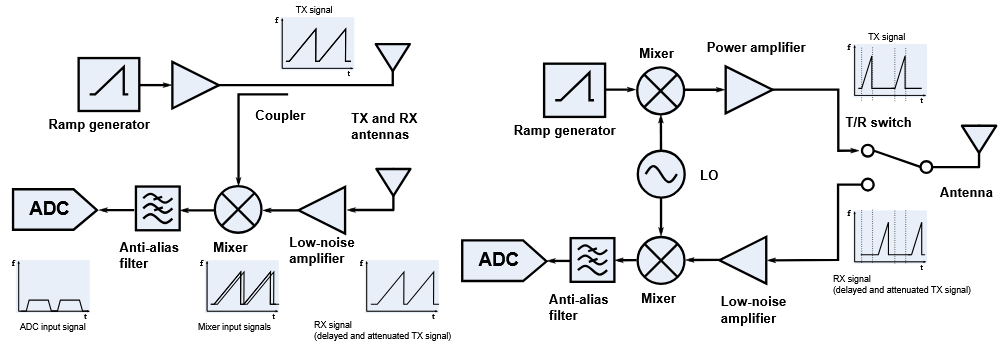
\includegraphics[width=0.6\textwidth]{src/rapport_complet/img/schéma block fmcw vs pulse.png}
    \caption{Schéma block FMCW (gauche) et pulse (droite)}
    \label{fig:image_schema_block}
\end{figure}

%TERMINER CA
Il existe également une variante du radar à impulsions qui comporte deux générateurs de rampe, l'un pour la réception (RX) et l'autre pour l'émission (TX). Cela donne un signal IF à basse fréquence, comme avec le radar FMCW. Cette architecture est souvent utilisée sur les radars SAR, car elle permet d'obtenir une bande passante RF élevée sans nécessiter d'ADC à haute vitesse.

Étant donné que les radars à impulsions avec antenne commutée ne peuvent pas émettre et recevoir simultanément, la durée maximale des impulsions est limitée par le temps nécessaire à l'impulsion pour atteindre la cible et revenir. Avec une distance minimale de 100 m, par exemple, la durée maximale de l'impulsion pour ne perdre aucune partie de celle-ci n'est que de 670 ns. Comme le radar à impulsions doit répartir le temps de mesure entre l'émission et la réception, cela réduit la puissance d'émission moyenne et diminue le rapport signal/bruit. Un grand nombre d'impulsions très courtes complique également la formation de l'image. Le temps nécessaire à la formation de l'image SAR est proportionnel au nombre d'impulsions, et une durée d'impulsion maximale très courte nécessite d'en transmettre un très grand nombre pour obtenir une image avec un bon rapport signal/bruit.

Le radar FMCW peut émettre et recevoir simultanément, ce qui améliore le rapport signal/bruit. La longueur maximale du balayage n'est limitée que par les exigences de vitesse d'échantillonnage de l'ouverture synthétique, mais elle peut atteindre plusieurs centaines de µs. Contrairement au radar à impulsions, il existe également une exigence de longueur minimale de balayage, car le signal réfléchi est mélangé au signal émis et doit donc être reçu pendant que le balayage est encore en cours d'émission. Une longueur de balayage longue permet de collecter beaucoup plus de puissance réfléchie par balayage. Le radar à impulsions pourrait également utiliser des antennes TX et RX séparées afin que cela ne pose pas de problème, mais cela supprimerait ses avantages par rapport au radar FMCW, moins coûteux à mettre en œuvre. Des antennes d'émission et de réception séparées nécessitent plus d'espace, mais en raison de la grande longueur maximale, il devrait être possible de placer deux petites antennes côte à côte sous le drone.

En général, le radar FMCW présente un avantage pour les applications à courte portée et les plateformes à déplacement lent. Le radar à impulsions est nécessaire lorsque la portée requise est longue (plus de quelques kilomètres).

\subsubsection{Spécificités du SAR}

Dans la suite de la partie 3.1, les éléments étudiés porteront uniquement sur le contexte de l'étude : imagerie via radar SAR embarqué sur drone avec toutes les contraintes et exigences sous-jacentes.


\subsection{Sous-systèmes RF}

Source RF / Synthétiseur : VCO, PLL, DDS, stabilité de phase critique pour SAR.

Émetteur : modulateur FMCW ou impulsionnel, amplificateur de puissance (PA).

Récepteur : LNA, mélangeurs, filtres, amplificateurs IF, démodulateur IQ.

Conversion fréquence / Base bande : downconversion, ADC haute dynamique.


\subsection{Antenne et front-end RF}

Antennes à ouverture synthétique : antennes linéaires, réseaux patch, antennes conformes.

Contraintes d’intégration (taille, masse, diagramme de rayonnement, polarisation).

Antennes actives vs passives, antennes MIMO pour SAR.


\subsection{Gestion des données}

Débits très élevés (plusieurs centaines de Mo/s).

Stockage embarqué (SSD industriels) ou transfert vers station au sol.


\subsection{Alimentation et contraintes embarquées}

Gestion énergétique, rendement RF.

Dissipation thermique, miniaturisation et fiabilité.